\documentclass{beamer}

\usepackage[utf8x]{inputenc}
\usepackage[romanian]{babel}
\usepackage{color}
\usepackage{alltt}
\usepackage{hyperref}
\usepackage{code/highlight}
\mode<presentation>
\usetheme{CDL}

\title[Object Oriented Programming]{Object Oriented Programming}
\subtitle{CDL - cursul 2}
\institute{ROSEdu}
\author{Adrian Scoică\\\,\,{adrian.sc@rosedu.org}}

\begin{document}

\setbeamertemplate{frametitle continuation}[from second]
\setbeamertemplate{footline}[frame number]

\frame{\titlepage}

\frame{\tableofcontents}

\section{Ce este OOP?}
    \frame{\tableofcontents[currentsection]}
    
    \begin{frame}{Despre concept}
    \begin{itemize}
    \setlength{\itemsep}{0.8cm}
    \item "O paradigmă de programare care folosește obiecte pentru a modela aplicații" \pause
    \item O modalitate de a structura mai modular logica unei aplicații \pause
    \item Face {\bf limbajele} mai flexibile și codul mai intuitiv \pause
    \item Noțiuni centrale: \pause
    	\begin{itemize}
    	\item clasă \pause
    	\item obiect \pause
    	\item moștenire \pause
    	\item încapsulare \pause
    	\item polimorfism \pause
    	\end{itemize}
    \end{itemize}
    \end{frame}

    \begin{frame}{Despre clase}
    \begin{itemize}
    \setlength{\itemsep}{0.4cm}
    \item Ce este o clasă? \pause
    \end{itemize}
    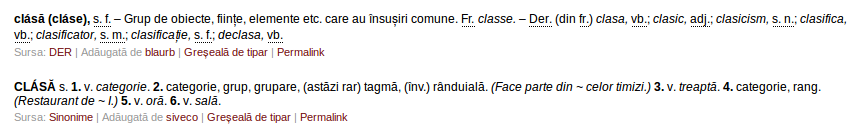
\includegraphics[scale=0.4]{Clasa.png}\\
    \pause Trăsăturile comune pot fi: \pause
	\begin{itemize} 
    \item structurale \pause 
    \item comportamentale 
    \end{itemize}
    \end{frame}

\section{În practică}
    \frame{\tableofcontents[currentsection]}

    \begin{frame}{Task: evidența populației}
    Vrem să implementăm un mecanism de a lucra cu o populație de "oameni" într-o aplicație (de exemplu, un joc). \pause Cerințe: \pause 
    \begin{itemize}
    \setlength{\itemsep}{0.5cm}
    \item Indivizii să aibă nume \pause
    \item Indivizii să aibă vârste diferite și sume de bani diferite \pause
    \item Indivizii să poată dona bani unii altora \pause
    \item Să putem ține evidența populației 
    \end{itemize}
    \end{frame}

    \begin{frame}{Soluția clasică}
    \pause \noindent
\ttfamily
\footnotesize
\hlstd{}\hlline{\ \ \ \ 1\ }\hlkwb{struct\ }\hlstd{Player}\hlsym{\{}\\
\hlline{\ \ \ \ 2\ }\hlstd{}\hlstd{\ \ \ \ \ \ \ \ }\hlstd{}\hlkwb{char\ }\hlstd{}\hlsym{{*}\ }\hlstd{name}\hlsym{;}\\
\hlline{\ \ \ \ 3\ }\hlstd{}\hlstd{\ \ \ \ \ \ \ \ }\hlstd{}\hlkwb{int\ }\hlstd{age}\hlsym{,\ }\hlstd{gold}\hlsym{;}\\
\hlline{\ \ \ \ 4\ }\hlstd{}\hlsym{\};}\\
\hlline{\ \ \ \ 5\ }\hlstd{}\hlkwb{int\ }\hlstd{Player\textunderscore count\ }\hlsym{=\ }\hlstd{}\hlnum{0}\hlstd{}\hlsym{;}\\
\hlline{\ \ \ \ 6\ }\hlstd{}\hlkwb{void\ }\hlstd{}\hlkwd{init\textunderscore P}\hlstd{}\hlsym{(}\hlstd{Player\ }\hlsym{{*}\ }\hlstd{player}\hlsym{,\ }\hlstd{}\hlkwb{char\ }\hlstd{}\hlsym{{*}\ }\hlstd{name}\hlsym{,\ }\hlstd{}\hlkwb{int\ }\hlstd{age}\hlsym{,\ }\hlstd{}\hlkwb{int\ }\hlstd{gold}\hlsym{)\{}\\
\hlline{\ \ \ \ 7\ }\hlstd{}\hlstd{\ \ \ \ \ \ \ \ }\hlstd{player}\hlsym{{-}$>$}\hlstd{name\ }\hlsym{=\ }\hlstd{}\hlkwd{strdup}\hlstd{}\hlsym{(}\hlstd{name}\hlsym{);}\\
\hlline{\ \ \ \ 8\ }\hlstd{}\hlstd{\ \ \ \ \ \ \ \ }\hlstd{player}\hlsym{{-}$>$}\hlstd{age\ }\hlsym{=\ }\hlstd{age}\hlsym{;\ }\\
\hlline{\ \ \ \ 9\ }\hlstd{}\hlstd{\ \ \ \ \ \ \ \ }\hlstd{player}\hlsym{{-}$>$}\hlstd{gold\ }\hlsym{=\ }\hlstd{gold}\hlsym{;}\\
\hlline{\ \ \ 10\ }\hlstd{}\hlsym{\}}\\
\hlline{\ \ \ 11\ }\hlstd{}\\
\hlline{\ \ \ 12\ }\hlkwb{void\ }\hlstd{}\hlkwd{donate}\hlstd{}\hlsym{(}\hlstd{Player\ }\hlsym{{*}\ }\hlstd{player}\hlsym{,\ }\hlstd{Player\ }\hlsym{{*}\ }\hlstd{dest}\hlsym{,\ }\hlstd{}\hlkwb{int\ }\hlstd{amount}\hlsym{)\{}\\
\hlline{\ \ \ 13\ }\hlstd{}\hlstd{\ \ \ \ \ \ \ \ }\hlstd{dest}\hlsym{{-}$>$}\hlstd{gold\ }\hlsym{+=\ }\hlstd{amount}\hlsym{;\ }\\
\hlline{\ \ \ 14\ }\hlstd{}\hlstd{\ \ \ \ \ \ \ \ }\hlstd{player}\hlsym{{-}$>$}\hlstd{gold\ }\hlsym{{-}=\ }\hlstd{amount}\hlsym{;}\\
\hlline{\ \ \ 15\ }\hlstd{}\hlsym{\}}\\
\hlline{\ \ \ 16\ }\hlstd{}\\
\hlline{\ \ \ 17\ }\hlkwb{void\ }\hlstd{}\hlkwd{print\textunderscore Player\ }\hlstd{}\hlsym{(}\hlstd{Player\ }\hlsym{{*}\ }\hlstd{player}\hlsym{,\ }\hlstd{}\hlkwb{FILE\ }\hlstd{}\hlsym{{*}\ }\hlstd{file}\hlsym{)\{}\\
\hlline{\ \ \ 18\ }\hlstd{}\hlstd{\ \ \ \ \ \ \ \ }\hlstd{}\hlkwd{fprintf}\hlstd{}\hlsym{(}\hlstd{f}\hlsym{,}\hlstd{}\hlstr{"Name:\ \%s}\hlesc{$\backslash$n}\hlstr{Age:\ \%d}\hlesc{$\backslash$n}\hlstr{Gold:\ \%d}\hlesc{$\backslash$n}\hlstr{"}\hlstd{}\hlsym{,\ }\\
\hlline{\ \ \ 19\ }\hlstd{}\hlstd{\ \ \ \ \ \ \ \ \ \ \ \ \ \ \ \ }\hlstd{player}\hlsym{{-}$>$}\hlstd{name}\hlsym{,\ }\hlstd{player}\hlsym{{-}$>$}\hlstd{age}\hlsym{,\ }\hlstd{player}\hlsym{{-}$>$}\hlstd{gold}\hlsym{);}\\
\hlline{\ \ \ 20\ }\hlstd{}\hlsym{\}}\hlstd{}\\
\mbox{}
\normalfont
\normalsize
\\
    \end{frame}

    \begin{frame}{Pas 1: Constructori}
    \pause \noindent
\ttfamily
\footnotesize
\hlstd{}\hlline{\ \ \ \ 1\ }\hlkwb{struct\ }\hlstd{Player}\hlsym{\{}\\
\hlline{\ \ \ \ 2\ }\hlstd{}\hlstd{\ \ \ \ \ \ \ \ }\hlstd{}\hlkwb{char\ }\hlstd{}\hlsym{{*}\ }\hlstd{name}\hlsym{;}\\
\hlline{\ \ \ \ 3\ }\hlstd{}\hlstd{\ \ \ \ \ \ \ \ }\hlstd{}\hlkwb{int\ }\hlstd{age}\hlsym{,\ }\hlstd{gold}\hlsym{;}\\
\hlline{\ \ \ \ 4\ }\hlstd{\\
\hlline{\ \ \ \ 5\ }}\hlstd{\ \ \ \ \ \ \ \ }\hlstd{}\hlkwd{Player}\hlstd{}\hlsym{(}\hlstd{}\hlkwb{char\ }\hlstd{}\hlsym{{*}\ }\hlstd{name}\hlsym{,\ }\hlstd{}\hlkwb{int\ }\hlstd{age}\hlsym{,\ }\hlstd{}\hlkwb{int\ }\hlstd{gold}\hlsym{)\ :\ }\\
\hlline{\ \ \ \ 6\ }\hlstd{}\hlstd{\ \ \ \ \ \ \ \ \ \ \ \ \ \ \ \ }\hlstd{}\hlkwd{name}\hlstd{}\hlsym{(}\hlstd{}\hlkwd{strdup}\hlstd{}\hlsym{(}\hlstd{name}\hlsym{)),\ }\hlstd{}\hlkwd{age}\hlstd{}\hlsym{(}\hlstd{age}\hlsym{),\ }\hlstd{}\hlkwd{gold}\hlstd{}\hlsym{(}\hlstd{gold}\hlsym{)\ \{\ \}}\\
\hlline{\ \ \ \ 7\ }\hlstd{}\hlsym{\};}\\
\hlline{\ \ \ \ 8\ }\hlstd{}\\
\hlline{\ \ \ \ 9\ }\hlkwb{int\ }\hlstd{Player\textunderscore count\ }\hlsym{=\ }\hlstd{}\hlnum{0}\hlstd{}\hlsym{;}\\
\hlline{\ \ \ 10\ }\hlstd{}\\
\hlline{\ \ \ 11\ }\hlkwb{void\ }\hlstd{}\hlkwd{donate}\hlstd{}\hlsym{(}\hlstd{Player\ }\hlsym{{*}\ }\hlstd{player}\hlsym{,\ }\hlstd{Player\ }\hlsym{{*}\ }\hlstd{dest}\hlsym{,\ }\hlstd{}\hlkwb{int\ }\hlstd{amount}\hlsym{)\{}\\
\hlline{\ \ \ 12\ }\hlstd{}\hlstd{\ \ \ \ \ \ \ \ }\hlstd{dest}\hlsym{{-}$>$}\hlstd{gold\ }\hlsym{+=\ }\hlstd{amount}\hlsym{;\ }\\
\hlline{\ \ \ 13\ }\hlstd{}\hlstd{\ \ \ \ \ \ \ \ }\hlstd{player}\hlsym{{-}$>$}\hlstd{gold\ }\hlsym{{-}=\ }\hlstd{amount}\hlsym{;}\\
\hlline{\ \ \ 14\ }\hlstd{}\hlsym{\}}\\
\hlline{\ \ \ 15\ }\hlstd{}\\
\hlline{\ \ \ 16\ }\hlkwb{void\ }\hlstd{}\hlkwd{print\textunderscore Player\ }\hlstd{}\hlsym{(}\hlstd{Player\ }\hlsym{{*}\ }\hlstd{player}\hlsym{,\ }\hlstd{}\hlkwb{FILE\ }\hlstd{}\hlsym{{*}\ }\hlstd{file}\hlsym{)\{}\\
\hlline{\ \ \ 17\ }\hlstd{}\hlstd{\ \ \ \ \ \ \ \ }\hlstd{}\hlkwd{fprintf}\hlstd{}\hlsym{(}\hlstd{f}\hlsym{,}\hlstd{}\hlstr{"Name:\ \%s}\hlesc{$\backslash$n}\hlstr{Age:\ \%d}\hlesc{$\backslash$n}\hlstr{Gold:\ \%d}\hlesc{$\backslash$n}\hlstr{"}\hlstd{}\hlsym{,\ }\\
\hlline{\ \ \ 18\ }\hlstd{}\hlstd{\ \ \ \ \ \ \ \ \ \ \ \ \ \ \ \ }\hlstd{player}\hlsym{{-}$>$}\hlstd{name}\hlsym{,\ }\hlstd{player}\hlsym{{-}$>$}\hlstd{age}\hlsym{,\ }\hlstd{player}\hlsym{{-}$>$}\hlstd{gold}\hlsym{);}\\
\hlline{\ \ \ 19\ }\hlstd{}\hlsym{\}}\hlstd{}\\
\mbox{}
\normalfont
\normalsize
\\
    \end{frame}
    
    \begin{frame}{Pas 2: Functii membru}
    \pause \noindent
\ttfamily
\footnotesize
\hlstd{}\hlline{\ \ \ \ 1\ }\hlkwb{struct\ }\hlstd{Player}\hlsym{\{}\\
\hlline{\ \ \ \ 2\ }\hlstd{}\hlstd{\ \ \ \ \ \ \ \ }\hlstd{}\hlkwb{char\ }\hlstd{}\hlsym{{*}\ }\hlstd{name}\hlsym{;}\\
\hlline{\ \ \ \ 3\ }\hlstd{}\hlstd{\ \ \ \ \ \ \ \ }\hlstd{}\hlkwb{int\ }\hlstd{age}\hlsym{,\ }\hlstd{gold}\hlsym{;}\\
\hlline{\ \ \ \ 4\ }\hlstd{\\
\hlline{\ \ \ \ 5\ }}\hlstd{\ \ \ \ \ \ \ \ }\hlstd{}\hlkwd{Player}\hlstd{}\hlsym{(}\hlstd{}\hlkwb{char\ }\hlstd{}\hlsym{{*}\ }\hlstd{name}\hlsym{,\ }\hlstd{}\hlkwb{int\ }\hlstd{age}\hlsym{,\ }\hlstd{}\hlkwb{int\ }\hlstd{gold}\hlsym{)\ :\ }\\
\hlline{\ \ \ \ 6\ }\hlstd{}\hlstd{\ \ \ \ \ \ \ \ \ \ \ \ \ \ \ \ }\hlstd{}\hlkwd{name}\hlstd{}\hlsym{(}\hlstd{}\hlkwd{strdup}\hlstd{}\hlsym{(}\hlstd{name}\hlsym{)),\ }\hlstd{}\hlkwd{age}\hlstd{}\hlsym{(}\hlstd{age}\hlsym{),\ }\hlstd{}\hlkwd{gold}\hlstd{}\hlsym{(}\hlstd{gold}\hlsym{)\ \{\ \}}\\
\hlline{\ \ \ \ 7\ }\hlstd{}\hlstd{\ \ \ \ \ \ \ \ \ \ \ \ \ \ \ \ }\hlstd{\\
\hlline{\ \ \ \ 8\ }}\hlstd{\ \ \ \ \ \ \ \ }\hlstd{}\hlkwb{void\ }\hlstd{}\hlkwd{donate}\hlstd{}\hlsym{(}\hlstd{Player\ }\hlsym{{*}\ }\hlstd{dest}\hlsym{,\ }\hlstd{amount}\hlsym{)\ \{}\\
\hlline{\ \ \ \ 9\ }\hlstd{}\hlstd{\ \ \ \ \ \ \ \ \ \ \ \ \ \ \ \ }\hlstd{dest}\hlsym{{-}$>$}\hlstd{gold\ }\hlsym{+=\ }\hlstd{amount}\hlsym{;}\\
\hlline{\ \ \ 10\ }\hlstd{}\hlstd{\ \ \ \ \ \ \ \ \ \ \ \ \ \ \ \ }\hlstd{gold\ }\hlsym{{-}=\ }\hlstd{amount}\hlsym{;}\\
\hlline{\ \ \ 11\ }\hlstd{}\hlstd{\ \ \ \ \ \ \ \ }\hlstd{}\hlsym{\}}\\
\hlline{\ \ \ 12\ }\hlstd{}\hlsym{\};}\\
\hlline{\ \ \ 13\ }\hlstd{}\\
\hlline{\ \ \ 14\ }\hlkwb{int\ }\hlstd{Player\textunderscore count\ }\hlsym{=\ }\hlstd{}\hlnum{0}\hlstd{}\hlsym{;}\\
\hlline{\ \ \ 15\ }\hlstd{}\\
\hlline{\ \ \ 16\ }\hlkwb{void\ }\hlstd{}\hlkwd{print\textunderscore Player\ }\hlstd{}\hlsym{(}\hlstd{Player\ }\hlsym{{*}\ }\hlstd{player}\hlsym{,\ }\hlstd{}\hlkwb{FILE\ }\hlstd{}\hlsym{{*}\ }\hlstd{file}\hlsym{)\{}\\
\hlline{\ \ \ 17\ }\hlstd{}\hlstd{\ \ \ \ \ \ \ \ }\hlstd{}\hlkwd{fprintf}\hlstd{}\hlsym{(}\hlstd{f}\hlsym{,}\hlstd{}\hlstr{"Name:\ \%s}\hlesc{$\backslash$n}\hlstr{Age:\ \%d}\hlesc{$\backslash$n}\hlstr{Gold:\ \%d}\hlesc{$\backslash$n}\hlstr{"}\hlstd{}\hlsym{,\ }\\
\hlline{\ \ \ 18\ }\hlstd{}\hlstd{\ \ \ \ \ \ \ \ \ \ \ \ \ \ \ \ }\hlstd{player}\hlsym{{-}$>$}\hlstd{name}\hlsym{,\ }\hlstd{player}\hlsym{{-}$>$}\hlstd{age}\hlsym{,\ }\hlstd{player}\hlsym{{-}$>$}\hlstd{gold}\hlsym{);}\\
\hlline{\ \ \ 19\ }\hlstd{}\hlsym{\}}\hlstd{}\\
\mbox{}
\normalfont
\normalsize
\\
    \end{frame}
    
    \begin{frame}{Pas 3: Variabile statice}
    \pause \noindent
\ttfamily
\footnotesize
\hlstd{}\hlline{\ \ \ \ 1\ }\hlkwb{struct\ }\hlstd{Player}\hlsym{\{}\\
\hlline{\ \ \ \ 2\ }\hlstd{}\hlstd{\ \ \ \ \ \ \ \ }\hlstd{}\hlkwb{char\ }\hlstd{}\hlsym{{*}\ }\hlstd{name}\hlsym{;}\\
\hlline{\ \ \ \ 3\ }\hlstd{}\hlstd{\ \ \ \ \ \ \ \ }\hlstd{}\hlkwb{int\ }\hlstd{age}\hlsym{,\ }\hlstd{gold}\hlsym{;}\\
\hlline{\ \ \ \ 4\ }\hlstd{}\hlstd{\ \ \ \ \ \ \ \ }\hlstd{}\hlkwb{static\ int\ }\hlstd{count}\hlsym{;}\\
\hlline{\ \ \ \ 5\ }\hlstd{\\
\hlline{\ \ \ \ 6\ }}\hlstd{\ \ \ \ \ \ \ \ }\hlstd{}\hlkwd{Player}\hlstd{}\hlsym{(}\hlstd{}\hlkwb{char\ }\hlstd{}\hlsym{{*}\ }\hlstd{name}\hlsym{,\ }\hlstd{}\hlkwb{int\ }\hlstd{age}\hlsym{,\ }\hlstd{}\hlkwb{int\ }\hlstd{gold}\hlsym{)\ :\ }\\
\hlline{\ \ \ \ 7\ }\hlstd{}\hlstd{\ \ \ \ \ \ \ \ }\hlstd{}\hlkwd{name}\hlstd{}\hlsym{(}\hlstd{}\hlkwd{strdup}\hlstd{}\hlsym{(}\hlstd{name}\hlsym{)),\ }\hlstd{}\hlkwd{age}\hlstd{}\hlsym{(}\hlstd{age}\hlsym{),\ }\hlstd{}\hlkwd{gold}\hlstd{}\hlsym{(}\hlstd{gold}\hlsym{)\ \{\ }\hlstd{count}\hlsym{++;\ \}}\\
\hlline{\ \ \ \ 8\ }\hlstd{}\hlstd{\ \ \ \ \ \ \ \ \ \ \ \ \ \ \ \ }\hlstd{\\
\hlline{\ \ \ \ 9\ }}\hlstd{\ \ \ \ \ \ \ \ }\hlstd{}\hlkwb{void\ }\hlstd{}\hlkwd{donate}\hlstd{}\hlsym{(}\hlstd{Player\ }\hlsym{{*}\ }\hlstd{dest}\hlsym{,\ }\hlstd{amount}\hlsym{)\ \{}\\
\hlline{\ \ \ 10\ }\hlstd{}\hlstd{\ \ \ \ \ \ \ \ \ \ \ \ \ \ \ \ }\hlstd{dest}\hlsym{{-}$>$}\hlstd{gold\ }\hlsym{+=\ }\hlstd{amount}\hlsym{;}\\
\hlline{\ \ \ 11\ }\hlstd{}\hlstd{\ \ \ \ \ \ \ \ \ \ \ \ \ \ \ \ }\hlstd{gold\ }\hlsym{{-}=\ }\hlstd{amount}\hlsym{;}\\
\hlline{\ \ \ 12\ }\hlstd{}\hlstd{\ \ \ \ \ \ \ \ }\hlstd{}\hlsym{\}}\\
\hlline{\ \ \ 13\ }\hlstd{}\hlsym{\};}\\
\hlline{\ \ \ 14\ }\hlstd{}\\
\hlline{\ \ \ 15\ }\hlkwb{int\ }\hlstd{Player}\hlsym{::}\hlstd{count\ }\hlsym{=\ }\hlstd{}\hlnum{0}\hlstd{}\hlsym{;}\\
\hlline{\ \ \ 16\ }\hlstd{}\\
\hlline{\ \ \ 17\ }\hlkwb{void\ }\hlstd{}\hlkwd{print\textunderscore Player\ }\hlstd{}\hlsym{(}\hlstd{Player\ }\hlsym{{*}\ }\hlstd{player}\hlsym{,\ }\hlstd{}\hlkwb{FILE\ }\hlstd{}\hlsym{{*}\ }\hlstd{file}\hlsym{)\{}\\
\hlline{\ \ \ 18\ }\hlstd{}\hlstd{\ \ \ \ \ \ \ \ }\hlstd{}\hlkwd{fprintf}\hlstd{}\hlsym{(}\hlstd{f}\hlsym{,}\hlstd{}\hlstr{"Name:\ \%s}\hlesc{$\backslash$n}\hlstr{Age:\ \%d}\hlesc{$\backslash$n}\hlstr{Gold:\ \%d}\hlesc{$\backslash$n}\hlstr{"}\hlstd{}\hlsym{,\ }\\
\hlline{\ \ \ 19\ }\hlstd{}\hlstd{\ \ \ \ \ \ \ \ \ \ \ \ \ \ \ \ }\hlstd{player}\hlsym{{-}$>$}\hlstd{name}\hlsym{,\ }\hlstd{player}\hlsym{{-}$>$}\hlstd{age}\hlsym{,\ }\hlstd{player}\hlsym{{-}$>$}\hlstd{gold}\hlsym{);}\\
\hlline{\ \ \ 20\ }\hlstd{}\hlsym{\}}\hlstd{}\\
\mbox{}
\normalfont
\normalsize
\\
    \end{frame}
    
    \begin{frame}{Pas 4: Operatori}
    \pause \noindent
\ttfamily
\footnotesize
\hlstd{}\hlline{\ \ \ \ 1\ }\hlkwb{struct\ }\hlstd{Player}\hlsym{\{}\\
\hlline{\ \ \ \ 2\ }\hlstd{}\hlstd{\ \ \ \ \ \ \ \ }\hlstd{}\hlkwb{char\ }\hlstd{}\hlsym{{*}\ }\hlstd{name}\hlsym{;}\\
\hlline{\ \ \ \ 3\ }\hlstd{}\hlstd{\ \ \ \ \ \ \ \ }\hlstd{}\hlkwb{int\ }\hlstd{age}\hlsym{,\ }\hlstd{gold}\hlsym{;}\\
\hlline{\ \ \ \ 4\ }\hlstd{}\hlstd{\ \ \ \ \ \ \ \ }\hlstd{}\hlkwb{static\ int\ }\hlstd{count}\hlsym{;}\\
\hlline{\ \ \ \ 5\ }\hlstd{\\
\hlline{\ \ \ \ 6\ }}\hlstd{\ \ \ \ \ \ \ \ }\hlstd{}\hlkwd{Player}\hlstd{}\hlsym{(}\hlstd{}\hlkwb{char\ }\hlstd{}\hlsym{{*}\ }\hlstd{name}\hlsym{,\ }\hlstd{}\hlkwb{int\ }\hlstd{age}\hlsym{,\ }\hlstd{}\hlkwb{int\ }\hlstd{gold}\hlsym{)\ :\ }\\
\hlline{\ \ \ \ 7\ }\hlstd{}\hlstd{\ \ \ \ \ \ \ \ }\hlstd{}\hlkwd{name}\hlstd{}\hlsym{(}\hlstd{}\hlkwd{strdup}\hlstd{}\hlsym{(}\hlstd{name}\hlsym{)),\ }\hlstd{}\hlkwd{age}\hlstd{}\hlsym{(}\hlstd{age}\hlsym{),\ }\hlstd{}\hlkwd{gold}\hlstd{}\hlsym{(}\hlstd{gold}\hlsym{)\ \{\ }\hlstd{count}\hlsym{++;\ \}}\\
\hlline{\ \ \ \ 8\ }\hlstd{}\hlstd{\ \ \ \ \ \ \ \ \ \ \ \ \ \ \ \ }\hlstd{\\
\hlline{\ \ \ \ 9\ }}\hlstd{\ \ \ \ \ \ \ \ }\hlstd{}\hlkwb{void\ }\hlstd{}\hlkwd{donate}\hlstd{}\hlsym{(}\hlstd{Player\ }\hlsym{{*}\ }\hlstd{dest}\hlsym{,\ }\hlstd{amount}\hlsym{)\ \{}\\
\hlline{\ \ \ 10\ }\hlstd{}\hlstd{\ \ \ \ \ \ \ \ \ \ \ \ \ \ \ \ }\hlstd{dest}\hlsym{{-}$>$}\hlstd{gold\ }\hlsym{+=\ }\hlstd{amount}\hlsym{;}\\
\hlline{\ \ \ 11\ }\hlstd{}\hlstd{\ \ \ \ \ \ \ \ \ \ \ \ \ \ \ \ }\hlstd{gold\ }\hlsym{{-}=\ }\hlstd{amount}\hlsym{;}\\
\hlline{\ \ \ 12\ }\hlstd{}\hlstd{\ \ \ \ \ \ \ \ }\hlstd{}\hlsym{\}}\\
\hlline{\ \ \ 13\ }\hlstd{}\hlsym{\};}\\
\hlline{\ \ \ 14\ }\hlstd{}\\
\hlline{\ \ \ 15\ }\hlkwb{int\ }\hlstd{Player}\hlsym{::}\hlstd{count\ }\hlsym{=\ }\hlstd{}\hlnum{0}\hlstd{}\hlsym{;}\\
\hlline{\ \ \ 16\ }\hlstd{\\
\hlline{\ \ \ 17\ }ostream}\hlsym{\&\ }\hlstd{}\hlkwc{operator}\hlstd{}\hlsym{$<$$<$\ (}\hlstd{ostream}\hlsym{\&\ }\hlstd{out}\hlsym{,\ }\hlstd{Player}\hlsym{\&\ }\hlstd{player}\hlsym{)\{}\\
\hlline{\ \ \ 18\ }\hlstd{}\hlstd{\ \ \ \ \ \ \ \ }\hlstd{}\hlkwa{return\ }\hlstd{out\ }\hlsym{$<$$<$\ }\hlstd{}\hlstr{"Name:\ "}\hlstd{\ }\hlsym{$<$$<$\ }\hlstd{name\ }\hlsym{$<$$<$\ }\hlstd{}\hlstr{"}\hlesc{$\backslash$n}\hlstr{Age:\ "}\hlstd{\ }\hlsym{$<$$<$\ }\hlstd{age\ \\
\hlline{\ \ \ 19\ }}\hlstd{\ \ \ \ \ \ \ \ \ \ \ \ \ \ \ \ }\hlstd{}\hlsym{$<$$<$\ }\hlstd{}\hlstr{"}\hlesc{$\backslash$n}\hlstr{Gold:\ "}\hlstd{\ }\hlsym{$<$$<$\ }\hlstd{gold\ }\hlsym{$<$$<$\ }\hlstd{}\hlstr{"}\hlesc{$\backslash$n}\hlstr{"}\hlstd{}\hlsym{;}\\
\hlline{\ \ \ 20\ }\hlstd{}\hlsym{\}}\hlstd{}\\
\mbox{}
\normalfont
\normalsize
\\
    \end{frame}
    
    \begin{frame}{Syntax sugar: Parametri Impliciti}
    \pause \noindent
\ttfamily
\footnotesize
\hlstd{}\hlline{\ \ \ \ 1\ }\hlkwb{struct\ }\hlstd{Player}\hlsym{\{}\\
\hlline{\ \ \ \ 2\ }\hlstd{}\hlstd{\ \ \ \ \ \ \ \ }\hlstd{}\hlkwb{char\ }\hlstd{}\hlsym{{*}\ }\hlstd{name}\hlsym{;}\\
\hlline{\ \ \ \ 3\ }\hlstd{}\hlstd{\ \ \ \ \ \ \ \ }\hlstd{}\hlkwb{int\ }\hlstd{age}\hlsym{,\ }\hlstd{gold}\hlsym{;}\\
\hlline{\ \ \ \ 4\ }\hlstd{}\hlstd{\ \ \ \ \ \ \ \ }\hlstd{}\hlkwb{static\ int\ }\hlstd{count}\hlsym{;}\\
\hlline{\ \ \ \ 5\ }\hlstd{\\
\hlline{\ \ \ \ 6\ }}\hlstd{\ \ \ \ \ \ \ \ }\hlstd{}\hlkwd{Player}\hlstd{}\hlsym{(}\hlstd{}\hlkwb{char\ }\hlstd{}\hlsym{{*}\ }\hlstd{name}\hlsym{,\ }\hlstd{}\hlkwb{int\ }\hlstd{age\ }\hlsym{=\ }\hlstd{}\hlnum{20}\hlstd{}\hlsym{,\ }\hlstd{}\hlkwb{int\ }\hlstd{gold\ }\hlsym{=\ }\hlstd{}\hlnum{0}\hlstd{}\hlsym{)\ :\ }\\
\hlline{\ \ \ \ 7\ }\hlstd{}\hlstd{\ \ \ \ \ \ \ \ }\hlstd{}\hlkwd{name}\hlstd{}\hlsym{(}\hlstd{}\hlkwd{strdup}\hlstd{}\hlsym{(}\hlstd{name}\hlsym{)),\ }\hlstd{}\hlkwd{age}\hlstd{}\hlsym{(}\hlstd{age}\hlsym{),\ }\hlstd{}\hlkwd{gold}\hlstd{}\hlsym{(}\hlstd{gold}\hlsym{)\ \{\ }\hlstd{count}\hlsym{++;\ \}}\\
\hlline{\ \ \ \ 8\ }\hlstd{}\hlstd{\ \ \ \ \ \ \ \ \ \ \ \ \ \ \ \ }\hlstd{\\
\hlline{\ \ \ \ 9\ }}\hlstd{\ \ \ \ \ \ \ \ }\hlstd{}\hlkwb{void\ }\hlstd{}\hlkwd{donate}\hlstd{}\hlsym{(}\hlstd{Player\ }\hlsym{{*}\ }\hlstd{dest}\hlsym{,\ }\hlstd{amount}\hlsym{)\ \{}\\
\hlline{\ \ \ 10\ }\hlstd{}\hlstd{\ \ \ \ \ \ \ \ \ \ \ \ \ \ \ \ }\hlstd{dest}\hlsym{{-}$>$}\hlstd{gold\ }\hlsym{+=\ }\hlstd{amount}\hlsym{;}\\
\hlline{\ \ \ 11\ }\hlstd{}\hlstd{\ \ \ \ \ \ \ \ \ \ \ \ \ \ \ \ }\hlstd{gold\ }\hlsym{{-}=\ }\hlstd{amount}\hlsym{;}\\
\hlline{\ \ \ 12\ }\hlstd{}\hlstd{\ \ \ \ \ \ \ \ }\hlstd{}\hlsym{\}}\\
\hlline{\ \ \ 13\ }\hlstd{}\hlsym{\};}\\
\hlline{\ \ \ 14\ }\hlstd{}\\
\hlline{\ \ \ 15\ }\hlkwb{int\ }\hlstd{Player}\hlsym{::}\hlstd{count\ }\hlsym{=\ }\hlstd{}\hlnum{0}\hlstd{}\hlsym{;}\\
\hlline{\ \ \ 16\ }\hlstd{\\
\hlline{\ \ \ 17\ }ostream}\hlsym{\&\ }\hlstd{}\hlkwc{operator}\hlstd{}\hlsym{$<$$<$\ (}\hlstd{ostream}\hlsym{\&\ }\hlstd{out}\hlsym{,\ }\hlstd{Player}\hlsym{\&\ }\hlstd{player}\hlsym{)\{}\\
\hlline{\ \ \ 18\ }\hlstd{}\hlstd{\ \ \ \ \ \ \ \ }\hlstd{}\hlkwa{return\ }\hlstd{out\ }\hlsym{$<$$<$\ }\hlstd{}\hlstr{"Name:\ "}\hlstd{\ }\hlsym{$<$$<$\ }\hlstd{name\ }\hlsym{$<$$<$\ }\hlstd{}\hlstr{"}\hlesc{$\backslash$n}\hlstr{Age:\ "}\hlstd{\ }\hlsym{$<$$<$\ }\hlstd{age\ \\
\hlline{\ \ \ 19\ }}\hlstd{\ \ \ \ \ \ \ \ \ \ \ \ \ \ \ \ }\hlstd{}\hlsym{$<$$<$\ }\hlstd{}\hlstr{"}\hlesc{$\backslash$n}\hlstr{Gold:\ "}\hlstd{\ }\hlsym{$<$$<$\ }\hlstd{gold\ }\hlsym{$<$$<$\ }\hlstd{}\hlstr{"}\hlesc{$\backslash$n}\hlstr{"}\hlstd{}\hlsym{;}\\
\hlline{\ \ \ 20\ }\hlstd{}\hlsym{\}}\hlstd{}\\
\mbox{}
\normalfont
\normalsize
\\
    \end{frame}

    \begin{frame}{Problem fix: Destructori}
    \pause \noindent
\ttfamily
\footnotesize
\hlstd{}\hlline{\ \ \ \ 1\ }\hlkwb{struct\ }\hlstd{Player}\hlsym{\{}\\
\hlline{\ \ \ \ 2\ }\hlstd{}\hlstd{\ \ \ \ \ \ \ \ }\hlstd{}\hlkwb{char\ }\hlstd{}\hlsym{{*}\ }\hlstd{name}\hlsym{;}\\
\hlline{\ \ \ \ 3\ }\hlstd{}\hlstd{\ \ \ \ \ \ \ \ }\hlstd{}\hlkwb{int\ }\hlstd{age}\hlsym{,\ }\hlstd{gold}\hlsym{;}\\
\hlline{\ \ \ \ 4\ }\hlstd{}\hlstd{\ \ \ \ \ \ \ \ }\hlstd{}\hlkwb{static\ int\ }\hlstd{count}\hlsym{;}\\
\hlline{\ \ \ \ 5\ }\hlstd{\\
\hlline{\ \ \ \ 6\ }}\hlstd{\ \ \ \ \ \ \ \ }\hlstd{}\hlkwd{Player}\hlstd{}\hlsym{(}\hlstd{}\hlkwb{char\ }\hlstd{}\hlsym{{*}\ }\hlstd{name}\hlsym{,\ }\hlstd{}\hlkwb{int\ }\hlstd{age\ }\hlsym{=\ }\hlstd{}\hlnum{20}\hlstd{}\hlsym{,\ }\hlstd{}\hlkwb{int\ }\hlstd{gold\ }\hlsym{=\ }\hlstd{}\hlnum{0}\hlstd{}\hlsym{)\ :\ }\\
\hlline{\ \ \ \ 7\ }\hlstd{}\hlstd{\ \ \ \ \ \ \ \ }\hlstd{}\hlkwd{name}\hlstd{}\hlsym{(}\hlstd{}\hlkwd{strdup}\hlstd{}\hlsym{(}\hlstd{name}\hlsym{)),\ }\hlstd{}\hlkwd{age}\hlstd{}\hlsym{(}\hlstd{age}\hlsym{),\ }\hlstd{}\hlkwd{gold}\hlstd{}\hlsym{(}\hlstd{gold}\hlsym{)\ \{\ }\hlstd{count}\hlsym{++;\ \}}\\
\hlline{\ \ \ \ 8\ }\hlstd{}\hlstd{\ \ \ \ \ \ \ \ }\hlstd{\\
\hlline{\ \ \ \ 9\ }}\hlstd{\ \ \ \ \ \ \ \ }\hlstd{}\hlkwc{virtual\ }\hlstd{}\hlsym{$\sim$}\hlstd{}\hlkwd{Player}\hlstd{}\hlsym{()\ \{\ }\hlstd{count}\hlsym{{-}{-};\ }\hlstd{}\hlkwd{free}\hlstd{}\hlsym{(}\hlstd{name}\hlsym{);\ \}}\hlstd{\ \ \ \ \ \ }\hlsym{}\\
\hlline{\ \ \ 10\ }\hlstd{}\hlstd{\ \ \ \ \ \ \ \ }\hlstd{\\
\hlline{\ \ \ 11\ }}\hlstd{\ \ \ \ \ \ \ \ }\hlstd{}\hlkwb{void\ }\hlstd{}\hlkwd{donate}\hlstd{}\hlsym{(}\hlstd{Player\ }\hlsym{{*}\ }\hlstd{dest}\hlsym{,\ }\hlstd{amount}\hlsym{)\ \{}\\
\hlline{\ \ \ 12\ }\hlstd{}\hlstd{\ \ \ \ \ \ \ \ \ \ \ \ \ \ \ \ }\hlstd{dest}\hlsym{{-}$>$}\hlstd{gold\ }\hlsym{+=\ }\hlstd{amount}\hlsym{;}\\
\hlline{\ \ \ 13\ }\hlstd{}\hlstd{\ \ \ \ \ \ \ \ \ \ \ \ \ \ \ \ }\hlstd{gold\ }\hlsym{{-}=\ }\hlstd{amount}\hlsym{;}\\
\hlline{\ \ \ 14\ }\hlstd{}\hlstd{\ \ \ \ \ \ \ \ }\hlstd{}\hlsym{\}}\\
\hlline{\ \ \ 15\ }\hlstd{}\hlsym{\};}\\
\hlline{\ \ \ 16\ }\hlstd{}\\
\hlline{\ \ \ 17\ }\hlkwb{int\ }\hlstd{Player}\hlsym{::}\hlstd{count\ }\hlsym{=\ }\hlstd{}\hlnum{0}\hlstd{}\hlsym{;}\\
\hlline{\ \ \ 18\ }\hlstd{}\\
\mbox{}
\normalfont
\normalsize
\\
    \end{frame}
    
    \begin{frame}{Safety fix: Accesul la membri}
    \pause \noindent
\ttfamily
\footnotesize
\hlstd{}\hlline{\ \ \ \ 1\ }\hlkwb{struct\ }\hlstd{Player}\hlsym{\{}\\
\hlline{\ \ \ \ 2\ }\hlstd{}\hlkwc{private}\hlstd{}\hlsym{:}\\
\hlline{\ \ \ \ 3\ }\hlstd{}\hlstd{\ \ \ \ \ \ \ \ }\hlstd{}\hlkwb{char\ }\hlstd{}\hlsym{{*}\ }\hlstd{name}\hlsym{;}\\
\hlline{\ \ \ \ 4\ }\hlstd{}\hlstd{\ \ \ \ \ \ \ \ }\hlstd{}\hlkwb{int\ }\hlstd{age}\hlsym{,\ }\hlstd{gold}\hlsym{;}\\
\hlline{\ \ \ \ 5\ }\hlstd{}\hlstd{\ \ \ \ \ \ \ \ }\hlstd{}\hlkwb{static\ int\ }\hlstd{count}\hlsym{;}\\
\hlline{\ \ \ \ 6\ }\hlstd{}\hlkwc{public}\hlstd{}\hlsym{:}\\
\hlline{\ \ \ \ 7\ }\hlstd{}\hlstd{\ \ \ \ \ \ \ \ }\hlstd{}\hlkwd{Player}\hlstd{}\hlsym{(}\hlstd{}\hlkwb{char\ }\hlstd{}\hlsym{{*}\ }\hlstd{name}\hlsym{,\ }\hlstd{}\hlkwb{int\ }\hlstd{age\ }\hlsym{=\ }\hlstd{}\hlnum{20}\hlstd{}\hlsym{,\ }\hlstd{}\hlkwb{int\ }\hlstd{gold\ }\hlsym{=\ }\hlstd{}\hlnum{0}\hlstd{}\hlsym{)\ :\ }\\
\hlline{\ \ \ \ 8\ }\hlstd{}\hlstd{\ \ \ \ \ \ \ \ }\hlstd{}\hlkwd{name}\hlstd{}\hlsym{(}\hlstd{}\hlkwd{strdup}\hlstd{}\hlsym{(}\hlstd{name}\hlsym{)),\ }\hlstd{}\hlkwd{age}\hlstd{}\hlsym{(}\hlstd{age}\hlsym{),\ }\hlstd{}\hlkwd{gold}\hlstd{}\hlsym{(}\hlstd{gold}\hlsym{)\ \{\ }\hlstd{count}\hlsym{++;\ \}}\\
\hlline{\ \ \ \ 9\ }\hlstd{}\hlstd{\ \ \ \ \ \ \ \ }\hlstd{}\hlkwc{virtual\ }\hlstd{}\hlsym{$\sim$}\hlstd{}\hlkwd{Player}\hlstd{}\hlsym{()\ \{\ }\hlstd{count}\hlsym{{-}{-};\ }\hlstd{}\hlkwd{free}\hlstd{}\hlsym{(}\hlstd{name}\hlsym{);\ \}}\hlstd{\ \ \ \ \ \ }\hlsym{}\\
\hlline{\ \ \ 10\ }\hlstd{}\hlstd{\ \ \ \ \ \ \ \ }\hlstd{}\hlkwb{void\ }\hlstd{}\hlkwd{donate}\hlstd{}\hlsym{(}\hlstd{Player\ }\hlsym{{*}\ }\hlstd{dest}\hlsym{,\ }\hlstd{amount}\hlsym{)\ \{}\\
\hlline{\ \ \ 11\ }\hlstd{}\hlstd{\ \ \ \ \ \ \ \ \ \ \ \ \ \ \ \ }\hlstd{dest}\hlsym{{-}$>$}\hlstd{gold\ }\hlsym{+=\ }\hlstd{amount}\hlsym{;}\\
\hlline{\ \ \ 12\ }\hlstd{}\hlstd{\ \ \ \ \ \ \ \ \ \ \ \ \ \ \ \ }\hlstd{gold\ }\hlsym{{-}=\ }\hlstd{amount}\hlsym{;}\\
\hlline{\ \ \ 13\ }\hlstd{}\hlstd{\ \ \ \ \ \ \ \ }\hlstd{}\hlsym{\}}\\
\hlline{\ \ \ 14\ }\hlstd{}\hlstd{\ \ \ \ \ \ \ \ }\hlstd{}\hlkwb{const\ char\ }\hlstd{}\hlsym{{*}\ }\hlstd{}\hlkwd{get\textunderscore name}\hlstd{}\hlsym{()\ \{\ }\hlstd{}\hlkwa{return\ }\hlstd{name}\hlsym{;\ \}}\\
\hlline{\ \ \ 15\ }\hlstd{}\hlstd{\ \ \ \ \ \ \ \ }\hlstd{}\hlkwb{int\ }\hlstd{}\hlkwd{get\textunderscore age}\hlstd{}\hlsym{()\ \{\ }\hlstd{}\hlkwa{return\ }\hlstd{age}\hlsym{;\ \}}\\
\hlline{\ \ \ 16\ }\hlstd{}\hlstd{\ \ \ \ \ \ \ \ }\hlstd{}\hlkwb{int\ }\hlstd{}\hlkwd{get\textunderscore gold}\hlstd{}\hlsym{()\ \{\ }\hlstd{}\hlkwa{return\ }\hlstd{gold}\hlsym{;\ \}}\\
\hlline{\ \ \ 17\ }\hlstd{}\hlstd{\ \ \ \ \ \ \ \ }\hlstd{}\hlkwb{static\ int\ }\hlstd{}\hlkwd{get\textunderscore count}\hlstd{}\hlsym{()\ \{\ }\hlstd{}\hlkwa{return\ }\hlstd{count}\hlsym{;\ \}}\\
\hlline{\ \ \ 18\ }\hlstd{}\hlsym{\};}\\
\hlline{\ \ \ 19\ }\hlstd{}\\
\hlline{\ \ \ 20\ }\hlkwb{int\ }\hlstd{Player}\hlsym{::}\hlstd{count\ }\hlsym{=\ }\hlstd{}\hlnum{0}\hlstd{}\hlsym{;}\hlstd{}\\
\mbox{}
\normalfont
\normalsize
\\
    \end{frame}
    
    \begin{frame}{New horizons: Moștenirea și supradefinirea}
    \pause \noindent
\ttfamily
\footnotesize
\hlstd{}\hlline{\ \ \ \ 1\ }\hlkwb{struct\ }\hlstd{Thief\ }\hlsym{:\ }\hlstd{}\hlkwc{public\ }\hlstd{Player\ }\hlsym{\{}\\
\hlline{\ \ \ \ 2\ }\hlstd{}\hlkwc{private}\hlstd{}\hlsym{:}\\
\hlline{\ \ \ \ 3\ }\hlstd{}\hlstd{\ \ \ \ \ \ \ \ }\hlstd{}\hlkwb{int\ }\hlstd{stolen}\hlsym{;}\\
\hlline{\ \ \ \ 4\ }\hlstd{}\hlkwc{public}\hlstd{}\hlsym{:}\\
\hlline{\ \ \ \ 5\ }\hlstd{}\hlstd{\ \ \ \ \ \ \ \ }\hlstd{}\hlkwd{Thief}\hlstd{}\hlsym{(}\hlstd{}\hlkwb{char\ }\hlstd{}\hlsym{{*}\ }\hlstd{name}\hlsym{,\ }\hlstd{}\hlkwb{int\ }\hlstd{age\ }\hlsym{=\ }\hlstd{}\hlnum{30}\hlstd{}\hlsym{,\ }\hlstd{}\hlkwb{int\ }\hlstd{gold\ }\hlsym{=\ }\hlstd{}\hlnum{0}\hlstd{}\hlsym{)\ :}\\
\hlline{\ \ \ \ 6\ }\hlstd{}\hlstd{\ \ \ \ \ \ \ \ \ \ \ \ \ \ \ \ }\hlstd{}\hlkwd{Player}\hlstd{}\hlsym{(}\hlstd{name}\hlsym{,\ }\hlstd{age}\hlsym{,\ }\hlstd{gold}\hlsym{),\ }\hlstd{}\hlkwd{stolen}\hlstd{}\hlsym{(}\hlstd{}\hlnum{0}\hlstd{}\hlsym{)\ \{\ \}}\\
\hlline{\ \ \ \ 7\ }\hlstd{}\hlstd{\ \ \ \ \ \ \ \ \ \ \ \ \ \ \ \ }\hlstd{\\
\hlline{\ \ \ \ 8\ }}\hlstd{\ \ \ \ \ \ \ \ }\hlstd{}\hlkwb{void\ }\hlstd{}\hlkwd{steal}\hlstd{}\hlsym{(}\hlstd{Player\ }\hlsym{{*}\ }\hlstd{player}\hlsym{,\ }\hlstd{}\hlkwb{int\ }\hlstd{amount}\hlsym{)\ \{}\\
\hlline{\ \ \ \ 9\ }\hlstd{}\hlstd{\ \ \ \ \ \ \ \ \ \ \ \ \ \ \ \ }\hlstd{player}\hlsym{{-}$>$}\hlstd{}\hlkwd{donate}\hlstd{}\hlsym{(}\hlstd{}\hlkwa{this}\hlstd{}\hlsym{,\ }\hlstd{amount}\hlsym{);}\\
\hlline{\ \ \ 10\ }\hlstd{}\hlstd{\ \ \ \ \ \ \ \ }\hlstd{}\hlsym{\}}\\
\hlline{\ \ \ 11\ }\hlstd{}\hlstd{\ \ \ \ \ \ \ \ }\hlstd{\\
\hlline{\ \ \ 12\ }}\hlstd{\ \ \ \ \ \ \ \ }\hlstd{}\hlkwb{void\ }\hlstd{}\hlkwd{donate}\hlstd{}\hlsym{(}\hlstd{Player\ }\hlsym{{*}\ }\hlstd{dest}\hlsym{,\ }\hlstd{amount}\hlsym{)\ \{\ }\\
\hlline{\ \ \ 13\ }\hlstd{}\hlstd{\ \ \ \ \ \ \ \ }\hlstd{}\hlsym{\}}\\
\hlline{\ \ \ 14\ }\hlstd{}\hlsym{\};}\hlstd{}\\
\mbox{}
\normalfont
\normalsize
\\
    \pause Dacă am vrea ca un Thief să se amestece printre Player, atunci trebuie să declarăm metoda din clasa de bază ca fiind virtuală!
    \end{frame}
    
\section{C++ cookies}
	\frame{\tableofcontents[currentsection]}
	\begin{frame}{STL: Introduction}
	STL este o bibliotecă (accesibilă printr-o serie de headere) standard din C++. \pause Conține: \pause
		\begin{itemize}
		\item Containere de date \pause
		\item Algoritmi \pause
		\end{itemize}
	Pe lângă STL, limbajul mai pune la dispoziție: \pause
		\begin{itemize}
		\item Metode de I/O \pause
		\item Clase pentru lucrul cu fișiere \pause
		\item {\bf Zeci} de alte îmbunătățiri
		\end{itemize}
	\end{frame}
	
	\begin{frame}{Exemplu utilizare: stringuri, lucrul cu fișiere}
	\noindent
\ttfamily
\footnotesize
\hlstd{}\hlline{\ \ \ \ 1\ }\hldir{\#include$<$iostream$>$}\\
\hlline{\ \ \ \ 2\ }\hlstd{}\hldir{\#include$<$string$>$}\\
\hlline{\ \ \ \ 3\ }\hlstd{}\\
\hlline{\ \ \ \ 4\ }\hlkwb{int\ }\hlstd{}\hlkwd{main}\hlstd{}\hlsym{()}\\
\hlline{\ \ \ \ 5\ }\hlstd{}\hlsym{\{}\\
\hlline{\ \ \ \ 6\ }\hlstd{}\hlstd{\ \ \ \ \ \ \ \ }\hlstd{std}\hlsym{::}\hlstd{string\ s1}\hlsym{,\ }\hlstd{s2}\hlsym{;}\\
\hlline{\ \ \ \ 7\ }\hlstd{}\hlstd{\ \ \ \ \ \ \ \ }\hlstd{std}\hlsym{::}\hlstd{cin\ }\hlsym{$>$$>$\ }\hlstd{s1\ }\hlsym{$>$$>$\ }\hlstd{s2}\hlsym{;}\\
\hlline{\ \ \ \ 8\ }\hlstd{}\hlstd{\ \ \ \ \ \ \ \ }\hlstd{\\
\hlline{\ \ \ \ 9\ }}\hlstd{\ \ \ \ \ \ \ \ }\hlstd{}\hlkwb{int\ }\hlstd{fromHere}\hlsym{;}\\
\hlline{\ \ \ 10\ }\hlstd{}\hlstd{\ \ \ \ \ \ \ \ }\hlstd{}\hlkwa{while\ }\hlstd{}\hlsym{((}\hlstd{fromHere\ }\hlsym{=\ }\hlstd{s1}\hlsym{.}\hlstd{}\hlkwd{find}\hlstd{}\hlsym{(}\hlstd{s2}\hlsym{))\ !=\ }\hlstd{std}\hlsym{::}\hlstd{string}\hlsym{::}\hlstd{npos}\hlsym{)\{}\\
\hlline{\ \ \ 11\ }\hlstd{}\hlstd{\ \ \ \ \ \ \ \ \ \ \ \ \ \ \ \ }\hlstd{s1}\hlsym{.}\hlstd{}\hlkwd{replace}\hlstd{}\hlsym{(}\hlstd{fromHere}\hlsym{,\ }\hlstd{s2}\hlsym{.}\hlstd{}\hlkwd{length}\hlstd{}\hlsym{(),\ }\hlstd{}\hlstr{""}\hlstd{}\hlsym{);}\\
\hlline{\ \ \ 12\ }\hlstd{}\hlstd{\ \ \ \ \ \ \ \ }\hlstd{}\hlsym{\}}\\
\hlline{\ \ \ 13\ }\hlstd{}\hlstd{\ \ \ \ \ \ \ \ }\hlstd{\\
\hlline{\ \ \ 14\ }}\hlstd{\ \ \ \ \ \ \ \ }\hlstd{std}\hlsym{::}\hlstd{cout\ }\hlsym{$<$$<$\ }\hlstd{s1\ }\hlsym{$<$$<$\ }\hlstd{std}\hlsym{::}\hlstd{endl}\hlsym{;}\\
\hlline{\ \ \ 15\ }\hlstd{}\hlstd{\ \ \ \ \ \ \ \ }\hlstd{\\
\hlline{\ \ \ 16\ }}\hlstd{\ \ \ \ \ \ \ \ }\hlstd{}\hlkwa{return\ }\hlstd{}\hlnum{0}\hlstd{}\hlsym{;}\\
\hlline{\ \ \ 17\ }\hlstd{}\hlsym{\}}\hlstd{}\\
\mbox{}
\normalfont
\normalsize

	\end{frame}
	
	\begin{frame}{Exemplu utilizare: vectori, algoritmi}
	\noindent
\ttfamily
\footnotesize
\hlstd{}\hlline{\ \ \ \ 1\ }\hldir{\#include$<$iostream$>$}\\
\hlline{\ \ \ \ 2\ }\hlstd{}\hldir{\#include$<$vector$>$}\\
\hlline{\ \ \ \ 3\ }\hlstd{}\hldir{\#include$<$algorithm$>$}\\
\hlline{\ \ \ \ 4\ }\hlstd{}\\
\hlline{\ \ \ \ 5\ }\hlkwb{int\ }\hlstd{}\hlkwd{main}\hlstd{}\hlsym{()}\\
\hlline{\ \ \ \ 6\ }\hlstd{}\hlsym{\{}\\
\hlline{\ \ \ \ 7\ }\hlstd{}\hlstd{\ \ \ \ \ \ \ \ }\hlstd{}\hlkwb{int\ }\hlstd{n}\hlsym{,\ }\hlstd{x}\hlsym{;}\\
\hlline{\ \ \ \ 8\ }\hlstd{}\hlstd{\ \ \ \ \ \ \ \ }\hlstd{std}\hlsym{::}\hlstd{vector}\hlsym{$<$}\hlstd{}\hlkwb{int}\hlstd{}\hlsym{$>$\ }\hlstd{v}\hlsym{;}\\
\hlline{\ \ \ \ 9\ }\hlstd{\\
\hlline{\ \ \ 10\ }}\hlstd{\ \ \ \ \ \ \ \ }\hlstd{}\hlkwa{for\ }\hlstd{}\hlsym{(}\hlstd{}\hlkwb{int\ }\hlstd{i\ }\hlsym{=\ }\hlstd{}\hlnum{0}\hlstd{}\hlsym{;\ }\hlstd{i\ }\hlsym{$<$\ }\hlstd{n}\hlsym{;\ }\hlstd{i}\hlsym{++)\{}\\
\hlline{\ \ \ 11\ }\hlstd{}\hlstd{\ \ \ \ \ \ \ \ \ \ \ \ \ \ \ \ }\hlstd{std}\hlsym{::}\hlstd{cin\ }\hlsym{$>$$>$\ }\hlstd{x}\hlsym{;}\\
\hlline{\ \ \ 12\ }\hlstd{}\hlstd{\ \ \ \ \ \ \ \ \ \ \ \ \ \ \ \ }\hlstd{v}\hlsym{.}\hlstd{}\hlkwd{push\textunderscore back}\hlstd{}\hlsym{(}\hlstd{x}\hlsym{);}\\
\hlline{\ \ \ 13\ }\hlstd{}\hlstd{\ \ \ \ \ \ \ \ }\hlstd{}\hlsym{\}}\\
\hlline{\ \ \ 14\ }\hlstd{}\hlstd{\ \ \ \ \ \ \ \ }\hlstd{\\
\hlline{\ \ \ 15\ }}\hlstd{\ \ \ \ \ \ \ \ }\hlstd{}\hlkwd{sort}\hlstd{}\hlsym{(}\hlstd{v}\hlsym{.}\hlstd{}\hlkwd{begin}\hlstd{}\hlsym{(),\ }\hlstd{v}\hlsym{.}\hlstd{}\hlkwd{end}\hlstd{}\hlsym{());\ }\hlstd{}\hlslc{//\ Dar\ descrescator??}\\
\hlline{\ \ \ 16\ }\hlstd{}\hlstd{\ \ \ \ \ \ \ \ }\hlstd{}\hlkwa{for\ }\hlstd{}\hlsym{(}\hlstd{}\hlkwb{int\ }\hlstd{i\ }\hlsym{=\ }\hlstd{}\hlnum{0}\hlstd{}\hlsym{;\ }\hlstd{i\ }\hlsym{$<$\ }\hlstd{n}\hlsym{;\ }\hlstd{i}\hlsym{++)\{}\\
\hlline{\ \ \ 17\ }\hlstd{}\hlstd{\ \ \ \ \ \ \ \ \ \ \ \ \ \ \ \ }\hlstd{std}\hlsym{::}\hlstd{cout\ }\hlsym{$<$$<$\ }\hlstd{v}\hlsym{{[}}\hlstd{i}\hlsym{{]}\ $<$$<$\ }\hlstd{}\hlstr{"\ "}\hlstd{}\hlsym{;}\\
\hlline{\ \ \ 18\ }\hlstd{}\hlstd{\ \ \ \ \ \ \ \ }\hlstd{}\hlsym{\}}\\
\hlline{\ \ \ 19\ }\hlstd{}\hlstd{\ \ \ \ \ \ \ \ }\hlstd{}\hlkwa{return\ }\hlstd{}\hlnum{0}\hlstd{}\hlsym{;}\\
\hlline{\ \ \ 20\ }\hlstd{}\hlsym{\}}\hlstd{}\\
\mbox{}
\normalfont
\normalsize

	\end{frame}

\section{Crearea unei Clase}
    \frame{\tableofcontents[currentsection]}

    \begin{frame}{Cerințe}
    Am vrea o clasă care să implementeze operații aritmetice cu numere complexe: \pause
    \begin{itemize}
    \setlength{\itemsep}{0.6cm}
    \item Clasa se va numi Complex \pause
    \item Constructorul va avea parametrii impliciți \pause
    \item Membrii de date vor fi privați \pause
    \item Avem la dispoziție funcții getter și funcție de aflat modulul \pause
    \item Avem un operator de adunare și unul de scădere
    \end{itemize}
    \end{frame}

\section{Link-uri Utile}
    \frame{\tableofcontents[currentsection]}

    \begin{frame}{Link-uri Utile}
    \begin{itemize}
    \setlength{\itemsep}{0.5cm}
    \footnotesize
    \item \url{http://www.cplusplus.com}{ - Sursa oficială de documentație a limbajului}
    \item \url{http://www.cs.brown.edu/\~jak/proglang/cpp/stltut/tut.html}{ - Un tutorial de bază pentru STL}
    \item \url{http://www.codeproject.com/KB/stl/stlintroduction.aspx}{ - Introducere în STL}
    \item \url{http://swarm.cs.pub.ro/~adrian.sc/PA/TutorialC++.pdf}{ - Tutorial C++ pentru programatorii de Java/C\#}
    \item \url{http://cdl.rosedu.org/2010/_media/cursuri/curs01/curs1_oop.pdf}{ - O prezentare mai detaliata despre OOP în C++ de la CDL 2010}
    \normalfont
    \end{itemize}
    \end{frame}
\end{document}
